\section{Iluminación Global}

Iluminación global se le llama al proceso de calcular la distribución de la energía de la luz sobre escenas tridimensionales desplegadas por computadora. Los efectos de la iluminación global incluyen suave sombreado debajo de objetos y cerca de esquinas, rebotes de luz, mezcla de colores, cáusticas, transluminiscencia, entre otros. Estos efectos son muy sutiles pero afectan el realismo de la imagen final de forma substancial \cite{pixar_renderman_intro}. La Figura \ref{fig:gi_comparison} muestra algunos de estos efectos.

\begin{figure}[H]
	\centering
	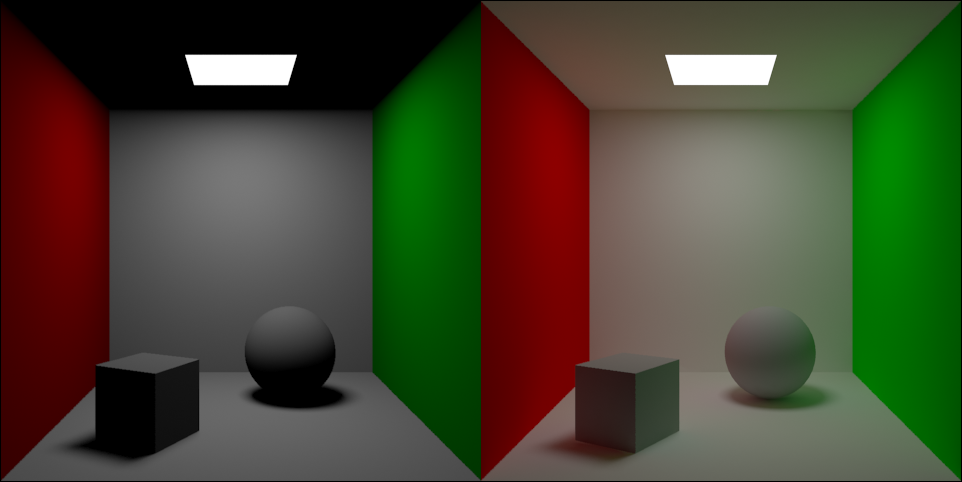
\includegraphics[width=0.985\linewidth]{media/direct_vs_indirect.png}
	\caption{Ejemplo de una escena con solo iluminación directa (izquierda). Iluminación global (derecha)}
	\label{fig:gi_comparison}
\end{figure}

El cómputo preciso y completo de iluminación global es considerado poco flexible, costoso y lento para ser utilizable en ciertos medios visuales que requieren producción de imágenes en tiempos interactivos o en escenas de gran complejidad, por ejemplo videojuegos o simulaciones. Es por ello que el desarrollo de aproximaciones y algoritmos para simular iluminación global con mejores factores de rendimiento y flexibilidad es un constante tema de investigación.
